O projeto dos controlador fuzzy foi focado na estabilização de atitude e altitude de um drone sujeito a parâmetros específicos\footnote{Estes valores foram também utilizados por \citeonline{Balas2007} para definir uma especificação do sistema}, sendo eles: a gravidade $g=9,81$ $m/s^2$, a massa do quadrotor $m=2,3$ $kg$ e o comprimento de cada haste do drone $l=0,5$ $m$. Um dos controladores projetado tem, como objetivo, controlar a altitude do drone, ao passo que um segundo visa a estabilização de sua atitude.

O controlador de altitude possui duas entradas e uma saída. As entradas são referentes à posição vertical do quadrotor ($z$) e sua respectiva velocidade ($\dot{z}$), ao passo que a saída diz respeito ao sinal de controle a ser aplicado sobre o sistema para estabilizar sua altitude ($u_1$). Sua aplicação no sistema é mostrada na Figura \ref{fig:u1_mamdani_blocks}.

% Mostrar diagrama do sistema controlado (para ruídos), sobre a entrada u1
\begin{figure}[!htb]
    \centering
    \caption{Diagrama do sistema de controle de altitude utilizando controlador fuzzy}
    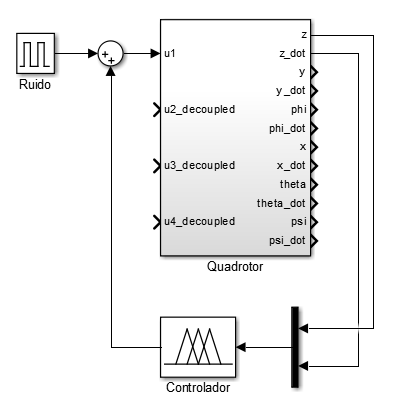
\includegraphics[width=0.5\textwidth]{./04-figuras/resultados/novos/simulink_printscreen_z}
    \label{fig:u1_mamdani_blocks}
\end{figure}

Utilizando o \textit{Fuzzy Logic Toolbox} do MATLAB, cada variável linguística do controlador fuzzy foi divida em três conjuntos: N (negativo), Z (zero) e P (positivo), baseado nos trabalhos de \citeonline{Maj2013} e \citeonline{Gao2014Stability}. As regras fuzzy definidas para este controlador são mostradas no Quadro \ref{qua:regras_fuzzy_u1_mamdani}, e a Figura \ref{fig:1_mamdani_surface} exibe seu equivalente em superfície.

% Mostrar regras Fuzzy envolvidas no controle de u1 (quadro de regras + superfície)
% Tá errada!
\begin{quadro}[!htb]
    \centering
    \caption{Regras fuzzy para modelagem do controle de altitude\label{qua:regras_fuzzy_u1_mamdani}}
    \begin{tabular}{|c|c|c|}
    % \begin{tabular}{>{\centering\bfseries}m{1in} >{\centering}m{1in}
        \hline
        \textbf{{$z$}} & 
        \textbf{{$\dot{z}$}} &
        \textbf{{$u_1$}} \\
        \hline %01
            N &
            - &
            N \\
        \hline %02
            P &
            - &
            P \\
        \hline %03
            Z &
            N &
            N \\
        \hline %04
            Z &
            Z &
            Z \\
        \hline %05
            Z &
            P &
            P \\
        \hline
    \end{tabular}
    % \begin{TAB}(r,1cm,2cm)[5pt]{|c|c|}{|c|c|c|}% (rows,min,max)[tabcolsep]{columns}{rows}
    %     hi & tall one    \\
    %     hi & medium one  \\
    %     hi & standard one\\
    % \end{TAB}
\end{quadro}


\begin{figure}[!htb]
    \centering
    \caption{Superfície das regras do sistema de controle fuzzy para a altitude do quadrotor}
    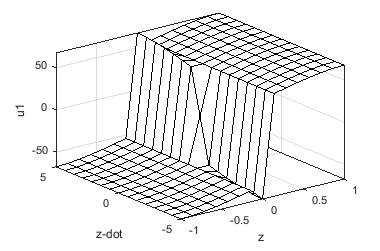
\includegraphics[width=0.6\textwidth]{./04-figuras/resultados/fis_u1/u1_mamdani_surface}
    \label{fig:1_mamdani_surface}
\end{figure}

O controlador de atitude projetado também possui duas entradas e uma saída. Desta vez, entretanto, as entradas são referentes ao ângulo em relação ao eixo horizontal ($\phi$ ou $\theta$) e sua respectiva variação ($\dot{\phi}$ ou $\dot{\theta}$). Mais uma vez, cada variável linguística foi dividida em três conjuntos: N, Z e P.

As regras que regem o controlador de atitude são sintetizadas no Quadro \ref{qua:regras_fuzzy_u2_u3_mamdani} e podem ser vistas na superfície de regras mostradas na Figura \ref{fig:u2_u3_mamdani_surface}.

% Mostrar regras Fuzzy envolvidas no controle de u2 e u3 (quadro de regras + superfície)
\begin{quadro}[!htb]
    \centering
    \caption{Regras fuzzy para modelagem do controle de atitude\label{qua:regras_fuzzy_u2_u3_mamdani}}
    \begin{tabular}{|c|c|c|}
    % \begin{tabular}{>{\centering\bfseries}m{1in} >{\centering}m{1in}
        \hline
        \textbf{{$\phi/\theta$}} & 
        \textbf{{$\dot{\phi}/\dot{\theta}$}} &
        \textbf{{$u_2/u_3$}} \\
        \hline %01
            P &
            P &
            N \\
        \hline %02
            P &
            Z &
            N \\
        \hline %03
            P &
            N &
            Z \\
        \hline %04
            N &
            N &
            P \\
        \hline %05
            N &
            Z &
            P \\
        \hline %06
            N &
            P &
            Z \\
        \hline %07
            Z &
            Z &
            Z \\
        \hline %08
            Z &
            N &
            P \\
        \hline %09
            Z &
            P &
            N \\
        \hline
    \end{tabular}
    % \begin{TAB}(r,1cm,2cm)[5pt]{|c|c|}{|c|c|c|}% (rows,min,max)[tabcolsep]{columns}{rows}
    %     hi & tall one    \\
    %     hi & medium one  \\
    %     hi & standard one\\
    % \end{TAB}
\end{quadro}


\begin{figure}[!htb]
    \centering
    \caption{Superfície das regras do sistema de controle fuzzy para a atitude do quadrotor}
    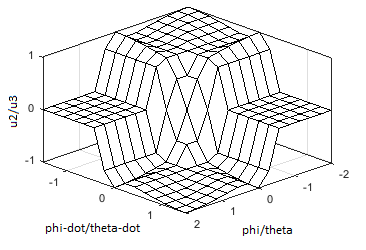
\includegraphics[width=0.6\textwidth]{./04-figuras/resultados/fis_u2/u2_u3_mamdani_surface}
    \label{fig:u2_u3_mamdani_surface}
\end{figure}

Já as Figuras \ref{fig:u2_mamdani_blocks} e \ref{fig:u3_mamdani_blocks} exibem os diagramas do sistema controlado, com atuação sobre os ângulos $\phi$ e $\theta$, respectivamente.

% Mostrar diagrama do sistema controlado (para ruídos), sobre as entradas u2 e u3
\begin{figure}[!htb]
    \centering
    \caption{Diagrama do sistema de controle de atitude utilizando controlador fuzzy sobre o ângulo $\phi$}
    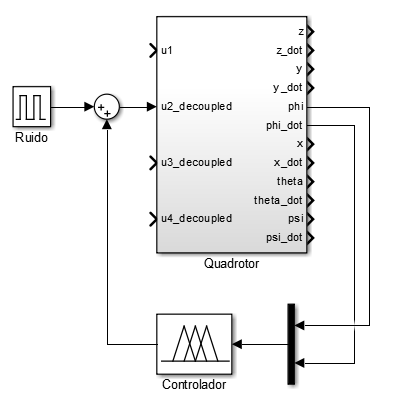
\includegraphics[width=0.6\textwidth]{./04-figuras/resultados/novos/simulink_printscreen_phi}
    \label{fig:u2_mamdani_blocks}
\end{figure}

\begin{figure}[!htb]
    \centering
    \caption{Diagrama do sistema de controle de atitude utilizando controlador fuzzy sobre o ângulo $\theta$}
    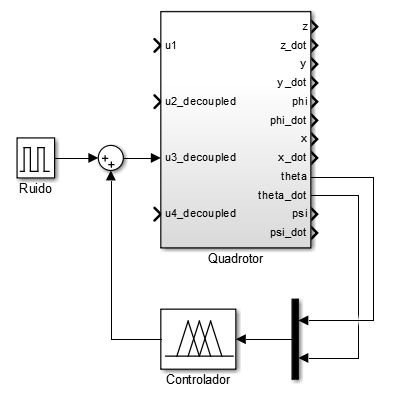
\includegraphics[width=0.5\textwidth]{./04-figuras/resultados/novos/simulink_printscreen_theta}
    \label{fig:u3_mamdani_blocks}
\end{figure}







